\documentclass{article}
\addtolength{\oddsidemargin}{-1.cm}
\addtolength{\textwidth}{2cm}
\addtolength{\topmargin}{-2cm}
\addtolength{\textheight}{3.5cm}
\newcommand{\HRule}{\rule{\linewidth}{0.5mm}}
\makeindex

\usepackage{longtable}
\usepackage[pdftex]{graphicx}
\usepackage{makeidx}
\usepackage{hyperref}
\usepackage{graphicx}
\graphicspath{ {images/}}


\usepackage{changepage,lipsum,titlesec}% http://ctan.org/pkg/{changepage,lipsum,titlesec}
\titleformat{\section}[block]{\bfseries}{\thesection.}{1em}{}
\titleformat{\subsection}[block]{}{\thesubsection}{1em}{}
\titleformat{\subsubsection}[block]{}{\thesubsubsection}{1em}{}
\titlespacing*{\subsection} {2em}{3.25ex plus 1ex minus .2ex}{1.5ex plus .2ex}
\titlespacing*{\subsubsection} {3em}{3.25ex plus 1ex minus .2ex}{1.5ex plus .2ex}

\setlength\parindent{74pt}

\hypersetup{
	colorlinks=true,
	linkcolor=black,
	filecolor=magenta,      
	urlcolor=cyan,
}


% define the title
\author{Team now.next}
\title{ Software Requirements Specification}
\begin{document}
	\setlength{\parskip}{6pt}
	
	% generates the title
	\begin{titlepage}
		
		\begin{center}
			% Upper part of the page       
			
			\textsc{\LARGE Department of Computer Science}\\[1.5cm]
			
			
\includegraphics{images/up-logo}
			
			\textsc{\Large COS 301 - Software Engineering}\\[0.5cm]
			% Title
			\HRule \\[0.4cm]
			%%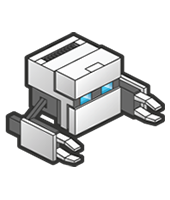
\includegraphics[width=0.05\textwidth]{./logo.png}\\[0.4cm] 
			{ \huge \bfseries Software Architecture Requirements Specification and Design}\\[0.4cm]
			\HRule \\[0.4cm]
			\textsc{\Large Team:  now.next()}\\[0.5cm]
			% Author and supervisor
			\begin{minipage}{0.4\textwidth}
				\begin{flushleft} \large
					\emph{Authors:}
				\end{flushleft}
			\end{minipage}
			\begin{minipage}{0.4\textwidth}
				\begin{flushright} \large
					\emph{Student number:}
				\end{flushright}
			\end{minipage}
			
			\begin{minipage}{0.4\textwidth}
				\begin{flushleft} \large
					Vuyani {Shabangu}
				\end{flushleft}
			\end{minipage}
			\begin{minipage}{0.4\textwidth}
				\begin{flushright} \large
					\emph{}
					11171139
				\end{flushright}
			\end{minipage}
			
			\begin{minipage}{0.4\textwidth}
				\begin{flushleft} \large
					Sibusiso {Masemola}
				\end{flushleft}
			\end{minipage}
			\begin{minipage}{0.4\textwidth}
				\begin{flushright} \large
					\emph{}
					12270467
				\end{flushright}
			\end{minipage}
			
			\begin{minipage}{0.4\textwidth}
				\begin{flushleft} \large
					Sello {Thosago}
				\end{flushleft}
			\end{minipage}
			\begin{minipage}{0.4\textwidth}
				\begin{flushright} \large
					\emph{}
					13062060
				\end{flushright}
			\end{minipage}
			
			\begin{minipage}{0.4\textwidth}
				\begin{flushleft} \large
					Banele {Nxumalo}
				\end{flushleft}
			\end{minipage}
			\begin{minipage}{0.4\textwidth}
				\begin{flushright} \large
					\emph{}
					12201911
				\end{flushright}
			\end{minipage}
			
			\begin{minipage}{0.4\textwidth}
				\begin{flushleft} \large
					Aiden {Malan}
				\end{flushleft}
			\end{minipage}
			\begin{minipage}{0.4\textwidth}
				\begin{flushright} \large
					\emph{}
					12265731
				\end{flushright}
			\end{minipage}
			
			
			\vfill
			
		\end{center}
	\end{titlepage}
	\footnotesize
	%\input{declaration_of_originality.tex}
	\normalsize
	
	
	\pagenumbering{roman}
	\tableofcontents
	\newpage
	\pagenumbering{arabic}
	
	\newpage %Aiden malan
	\section{Introduction} 
	The architectural requirements of the drone mission project will be discussed in this specification. There are number of quality control, safety and legal requirements that will be discussed in the following sections and the possible plans to implement them. It is important to understand the system inside and out so that we can create a system where all parties are covered and have some form of insurance in case of unforeseen circumstances and to prevent some of these circumstances from occurring.
	\begin{itemize} 
		\item The vision.
		\item The background.
	\end{itemize}
	
	\section{Vision}%%aiden
	The project aims to equip people who see a need for a drone. Without having to own a very expensive drone or have the expertise to operate the drone which can be as expensive to acquire. With the Drone Mission Project in full effect customers can achieve maximum output out of every mission while the business continues to reap in the rewards of the service portal we provide.
	
	
	\section{Background} %%aiden
	The Drone Mission project is aimed at equipping a client that would need the services of the drone but does not own a drone or the expertise to control the drone. The client or user would register to the website service and request the details of his mission such as time, place and if it is a recurring mission every hour, day, week, etc. The system would process all details and a drone operator will send information back to system to fly the drone. Information is captured and sent to the client efficiently.
	\newpage
	
	\section{Architecture Requirements}%Header
	\subsection{Architectural Scope}%%Aiden
	There are numerous quality requirements required from the system in order to operate the drones correctly to ensure safety of user, drone, client and organisation as a whole. These quality requirements range from the legal factors, safety of the drone in case of failure of any sort, client details protection and data safety and last but not least the safety of everyone around the use of the drone.
	%Here just talk about overview of the architectural requirements. Just broadly what the quality of the product must be.
	
	\setlength{\leftskip}{45px}
		
	\subsection{Quality Requirements}%%Vuyani
	The following is a list of quality requirements that have been established by the product owner that the system must posses.
	\subsubsection{Stability}
	\setlength{\leftskip}{61px}
	In order to avoid costly damage to the drones, the system must be stable in that it must not be susceptible to failure. Should the system controlling the drone fail, the system should be able to guarantee the safe landing of a drone.
	
	\subsubsection{Performance}
	All non-reporting operations such as user registration, user login, mission submission, mission display, operator mission setup should not take longer than 0.5 seconds.
	
	The reporting operation where a report is given to the user after the drone has performed a mission should not take longer than 5 seconds after the report data has been made available to the system.
	
	Network overhead has not been included in these figures because that is beyond the control of the system.
	
	\subsubsection{Privacy}
	Drone missions should only be permitted in areas that are allowed by South African legislation pertaining to the flying of Unmanned Aerial Vehicles.
	
	The missions performed by the drones must also be permitted by South African legislation.
	
	\subsubsection{Security}
	It is important that this system adheres to the highest security standards because it will be storing personal user information such as physical addresses, as well as allowing for the control of drones which are expensive and can be dangerous if in the wrong hands. Therefore the system has ensure that:
	\begin{itemize}
		\item Personal user data such as password is encrypted to remain hidden from unauthorised users and operators.
		\item Only authentified users are able to access the system
		\item Users only perform what they are authorised to do (e.g. users can only see their own mission information, users cannot perform operator operations).
		\item Data sent between web portal client and server should be encrypted.
		\item Connectivity to drones should only be limited to authorised and authentified users and system components
	\end{itemize}
	
	\subsubsection{Scalability}
	The system should scale up in order to be able to support a growing number of users, drone missions (which may be simultaneous), and drones. It should also scale as the data (user data, drone data and reporting data) held by the system increases.
	
	\subsubsection{Integration}
	The system must be able to interface with different drones.
	\subsection{Integration and Access Channel Requirements}%%Sello
	%Here just speak about what the system is expected to integrate with. Write about how it is suppose to be accessable to 			%web for users and operators.  It must also be able to interact with different types of drones.
	\subsubsection{Integration}
	The system has to work with the ArduPilot system, which is the the auto-pilot system for the drones. This ArduPilot system has to be connected to the PixHawk flight controller hardware, which is the hardware that is attached to and has physical control of the drones. The drone operating system should be able to deploy missions to as many different drones as possible.
	\subsubsection{Access Channels}
	The system is supposed to have a portal for drone users and operators which should be accessible through the internet. In the later stages of development, after completion of the web version of the system, the system could also possibly be made into an Android application.
	\subsection{Architectural Constraints }%%Banele
	%Talk about the constraints that we might have in producing the architecture that they have asked for.
	\begin{itemize}
		\item	The platform of the system will  be namely web application since we dealing with portal 
		\item	The database that will be used is mongoDB which favours JSON-like documents instead of table-based relation DB structure.
		\item 	Since the drones are built on an open source platform, the system will make use of Pixhawk autopilot for autonomous flight and Ardupilot mission planning software for command and control
		\item 	Since it is a website , HTML and javascript (both client and server side) will be used to built web application
	\end{itemize}
	
	\section{Architectural patterns}%%Sibusiso MVC, layered
	%Write that we are using a hybrid of MVC and Layered pattern (MVC to support the web part of the system, and layered to 		%support the intergability required by the part of the system that talks to the drones)
	
	\begin{itemize}
	
	\item Architectural pattern:
	MVC architectural pattern
	Model - nodeJS/mongoose
	View - portal/operator
	Controller- angularJS
	
	\item Layered architectural pattern
	
	
	 A hybrid architecture of MVC and the layered architecture has been adopted for this project. The MVC will be used to built the web application component of the system that interfaces with the users and operators. MVC was adopted because of how it easily facilitates good team work in web projects through the separation of concerns. 
	 
	 The Layered architecture will be used in component of the system that interact with the drones. It will consist of the same persistence resources used in the model of the MVC component, then the business layer and access layer will be built on top of that. This architecture has been chosen to fulfil the integration requirement which states that the system must be able to interface with different types of drones. This layered approach will allow us to encapsulate the control of different drone types and provide a consistent interface to the system.
	
	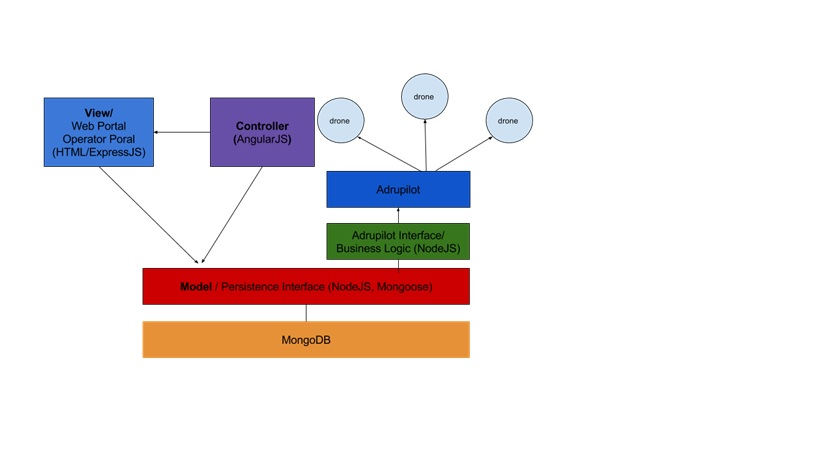
\includegraphics{images/MVCLayered}
	
	Figure 1. Hybrid of MVC-Layered pattern
	
	\end{itemize}
	
	
	
	
	\section{Architectural Tactics}%%Banele
	%use the same tactics that we spoke about in the presentation, discuss them more in detail
	\subsection{Scalability/Performance }
	Performance is an indication of how responsive a system is and how it goes about in executing specific actions in a given time and interval. It can be measured by in terms of latency and throughput.
	Latency is the time taken to respond to any event. Throughput is the number of events that take place in a given amount of time. Performance thus effects scalability, if the performance of application is high , then the scalability will be high as well. Performance can be achieved by the following tactics:
	\subsubsection{Increase Processing Power}
	Increasing processing power can be achieved by increasing number of Dynos on Heroku. A dyno is a lightweight Linux container that runs a single user-specified command. Dynos can be used to handle multiple jobs of the application . Dynos are like threads that can be assigned different jobs and each dyno can run a single process of the application.
	\subsection{Security}
	Security is about keeping user data secure and prevent illicit access to another user's mission details. In order security to be achieved , certain goals must be met like confidentiality, integrity and assurance.Security tactic can be broken down into the following architectural tactics: 
	\subsubsection{Authentication}
	It is about giving the right people access to the system. SSH certificates and passwords will provide authentication. The portal will provide the opportunity for users to enter login details and the details will then be authenticated by the system. 
	\subsubsection{Authorisation}
	Giving the authenticated people authority over only what they can do (Privacy). It is also about ensuring that an authenticated user has the rights to access and modify either data or services which includes selecting type of mission for the drone ,selecting the area by the drone and the date for the mission.
	
	\subsection{Integrability}
	Integrability is the ability to make the separately developed components of the system work correctly together. The drone management server should be able to interface with and control real drones. The drone operator must communicate well with web the server to ensure that the drones do specific missions appropriately. In order to provide access to other components of the system, the following tactic can be user:
	
	\subsubsection{Support Standard Communication Protocals}
	The system will make use of RESTful HTTP API.
	REST will ensure that the communication between the client which is the operator portal or the user portal and the server is well handled.
	
	\section{Access and Integration channels}%%Sello
	%This time, you are writing about the how we will meet the intergration requirements that you wrote about earlier. Write about how 	%we will use a HTTPS REST API to interact with the web portal. Talk about our layered approach to interacting with the drones; 	%our system->drone interfacing object -> adrupilot -> pixhawk -> drone.
	\subsection{Integration Channels}
	The drone user or operator portal will generate a text file. From this text file, an external drone operator will read the contents of the text file and enter the mission details into the ArduPilot software. The PixHawk flight controller hardware needs to be physically connected to the computer running the ArduPilot software via USB. The PixHawk flight controller keeps a stack of all ordered missions. The flight controller will then send the mission instructions to the drone via a wireless connection.
	\subsection{Access Channels}
	A HTTPS RESTful API will be used to handle the communication between the web client (the drone user or operator portal) and the web server. 
	
	\section{Frameworks}
	We have chosen to use the MEAN Stack framework which is a fullstack javascript framework which intuitively combines MongoDB , Express.js, AngularJS, NodeJS. We have chosen it because it perfectly puts together the technologies we have chosen for this project. and also fits in with the MVC architectural pattern that we had chosen. Each of the technologies bundled in the MEAN Stack are explained in the section below.
	
	
	\section{Technologies}%%Sibusiso
	%List and describe all the technologies we will be using, including why we are using them. Make sure for each one you mention 	%how it solves an architectural requirement.
	%MEAN Stack (Mongo, ExpressJS, AngualrJS, NodeJS), Mongoose (for ORM), Heroku Server, Travis for CI... and others
	
	 
	 The system will be Web based, so the technologies that will guide with building of the mentioned are:
	 
	 \begin{itemize}
	 	
	 	
	 	
	 	\item MongoDB - For the Database, MongoBD is a Cross-platform database, classified as a NoSQL database, This will be used to enter and store flexible data in document form in our database. flexible data will be needed in the system, it will allow to store wide range of mission types or a combination of them.
	 	
	 	Having a NoSQL database will benefit us since our database structure will be changing quite frequently based on frequent change and addition of requirements fro the client. MongoDB's ability to scale up when certain operations are requested frequently was another reason why we chose it as our primary persistence resource.
		
	 	\item Express - As the web framework, Express provides set of robust features for multi-page web development. Great for Accessibility as it consists of HTTP utility methods, it will help create a RESTFUL API in the system.
	 	
	 	
	 	\item AngularJS - As the front-end framework, AngularJs will be used for fast, efficient form validation on user side, aiding to easy server communication in the MEAN Stack, scaling up performance of system. AngularJS will allow us to focus on developing very user-friendly interfaces easily.
	 	
	 	\item NodeJS - The server platform, will be used for validating passed data before its passed on to be stored on database. command line  tool that will cater for  communication with MongoDb, the server, providing persistent connection from browser client to the server. in effect the system will be able to handle concurrent requests easier.
	 	
		We have chosen NodeJS because of it's asynchronous abilities which will be useful to fulfil the requirement that certain mission will have to be executed simultaneously. The fact that NodeJS was built on the V8 Javascript Engine which was built by Google for the Chromium Project gives us confidence in its high performance.
		
	 	\item Mongoose - This will be our Object Relational Mapping tool which will allow us to intuitively persist objects straight into the database. Mongoose will take care of mongoDB validation, casting and business logic side of the system. Catering for converting data between incompatible types, this promotes privacy and performance of the system.  
	 	
	 	
	 	\item Heroku Cloud Server - Hosting server, For cloud application platform, Heroku will be used for deployment, version control, and accessibility to the latest version from anywhere. Heroku provides a Platform-as-a-Service and we chose it specificically because of the ability to increase Dynos, which can scale up for multiple processing, since background and web applications are independently processed.
	 	
	 	\item Travis CI - for testing, this technology will be used to build and test the system, continuously; thus not allowing for any incorrect functionality to be incoporated to the system. aiding to the stability of the system as a whole.   
	 	
	 \end{itemize}
	 
	
	
	
	
\end{document}
